\documentclass[12pt]{beamer}
\setbeamertemplate{navigation symbols}{}
\usetheme{Copenhagen}
\usepackage{listings}
\usepackage{xcolor}
\usepackage{graphicx}
\usepackage{hyperref}
\graphicspath{ {imagenes/} }

\definecolor{codegreen}{rgb}{0,0.6,0}
\definecolor{codegray}{rgb}{0.5,0.5,0.5}
\definecolor{codepurple}{rgb}{0.58,0,0.82}
\definecolor{backcolour}{rgb}{0.95,0.95,0.92}

\lstdefinestyle{mystyle}{
    language=c++,
    backgroundcolor=\color{backcolour},   
    commentstyle=\color{codegreen},
    keywordstyle=\color{magenta},
    numberstyle=\tiny\color{codegray},
    stringstyle=\color{codepurple},
    basicstyle=\ttfamily\footnotesize,
    breakatwhitespace=false,         
    breaklines=true,                 
    captionpos=b,                    
    keepspaces=true,                 
    numbers=left,                    
    numbersep=5pt,                  
    showspaces=false,                
    showstringspaces=false,
    showtabs=false,                  
    tabsize=2
}

\lstset{style=mystyle}

\title{Arreglos en C++}
\subtitle{Operaciones}
\author{Tomás Peiretti}
\date{}

\begin{document}

\maketitle

\begin{frame}{Operaciones con arreglos}
    ¿Qué operaciones debemos saber realizar con los arreglos para aprobar AEDD?
    \begin{itemize}
        \item Recorrer (de izq a derecha, en un rango, de der a izq, etc)
        \item Invertir un arreglo
        \item Eliminar/agregar un elemento
        \item Buscar un elemento
        \item Ordenar (BubbleSort, MergeSort, SelectionSort, InsertionSort)
    \end{itemize}
\end{frame}

\begin{frame}[fragile]{Recorrer un arreglo}
\begin{lstlisting}[basicstyle=\tiny]
void recorrerCompleto(const int arr[], int tam) {
    for(int i=0; i<tam; i++) {
        cout << arr[i] << endl;
    }
}

void recorrerEnRango(const int arr[], int a, int b) {
    for (int i=a; i<=b; i++) {
        cout << arr[i] << endl;
    }
}

void recorrerCompletoAlReves(const int arr[], int tam) {
    for(int i = tam-1 ; i>=0 ; i--) {
        cout << arr[i] << endl;
    }
}

void recorrerHaciaElCentro(const int arr[], int tam) {
    int izq = 0, der = tam - 1;
    while (izq < der) {
        cout << "arr[" << izq << "] = " << arr[izq] << endl;
        cout << "arr[" << der << "] = " << arr[der] << endl;
        izq++;
        der--;
    }
    // elemento del medio
    if (tam%2 != 0)
        cout << "arr[" << tam/2 << "] = " << arr[tam/2] << endl;
}

\end{lstlisting}
\end{frame}

\begin{frame}[fragile]{Invertir un arreglo}
\begin{lstlisting}[basicstyle=\scriptsize]
void invertirConCopia(int arr[], int tl) {

    int copia[100000];
    for (int i=0; i<tl; i++) {
        copia[tl-1 - i] = arr[i];
    }

    for (int i=0; i<tl; i++) {
        arr[i] = copia[i];
    }
}

void invertir(int arr[], int tl) {

    int izq = 0, der = tl-1;
    
    while(izq <= der) {
        swap(arr[izq], arr[der]);
        izq++;
        der--;
    }
}
\end{lstlisting}
\end{frame}

\begin{frame}[fragile]{Eliminar un elemento del arreglo}
\begin{lstlisting}[basicstyle=\scriptsize]
// elimina el elemento que 
// se encuentra en la posicion indicada
void eliminarElemento(char arr[], int &tl, int posicion) {
    
    if (tl == 0)
        cout << "ERROR! no hay elementos para eliminar";
    else if (posicion >= tl)
        cout << "ERROR! posicion invalida";
    else {
        // borrar un elemento implica desplazar todos los 
        // elementos que estaban a su derecha
        // una posicion a la izquierda
        for (int i=posicion; i<tl-1; i++) {
            arr[i] = arr[i+1];
        }
        // y no hay que olvidarse de actualizar
        // el tamanioo logico
        tl--;
    }
}
\end{lstlisting}
\end{frame}
    
\begin{frame}[fragile]{Agregar un elemento al arreglo}
\begin{lstlisting}[basicstyle=\tiny]
#define TF 1500

// agrega el elemento en la posicion indicada
void agregarElemento(int arr[], int &tl, int posicion, int elemento) {
    
    if (tl == TF)
        cout <<"ERROR! ya no queda espacio";
    else if (posicion > tl)
        cout << "ERROR! posicion invalida";
    else {
        // agregar un elemento implica desplazar todos los 
        // elementos que se encuentran de la posicion en adelante
        // una posicion a la derecha
        // (primero hay que darle lugar al nuevo elemento)
        for (int i=tl; i>=posicion; i--) {
            arr[i+1] = arr[i];
        }
        //luego hay que agregar el elemento
        arr[posicion] = elemento;
        // y no hay que olvidarse de actualizar
        // el tamanioo logico
        tl++;
    }
}
\end{lstlisting}
\end{frame}

\begin{frame}{Buscar un elemento}
    Una de las operaciones que más utilizaremos es la \alert{búsqueda} de cierto elemento dentro de un arreglo.
    
    \medskip
    
    Supongamos que queremos buscar dentro del siguiente arreglo de enteros el número \alert{1253}
    
    \medskip
    
    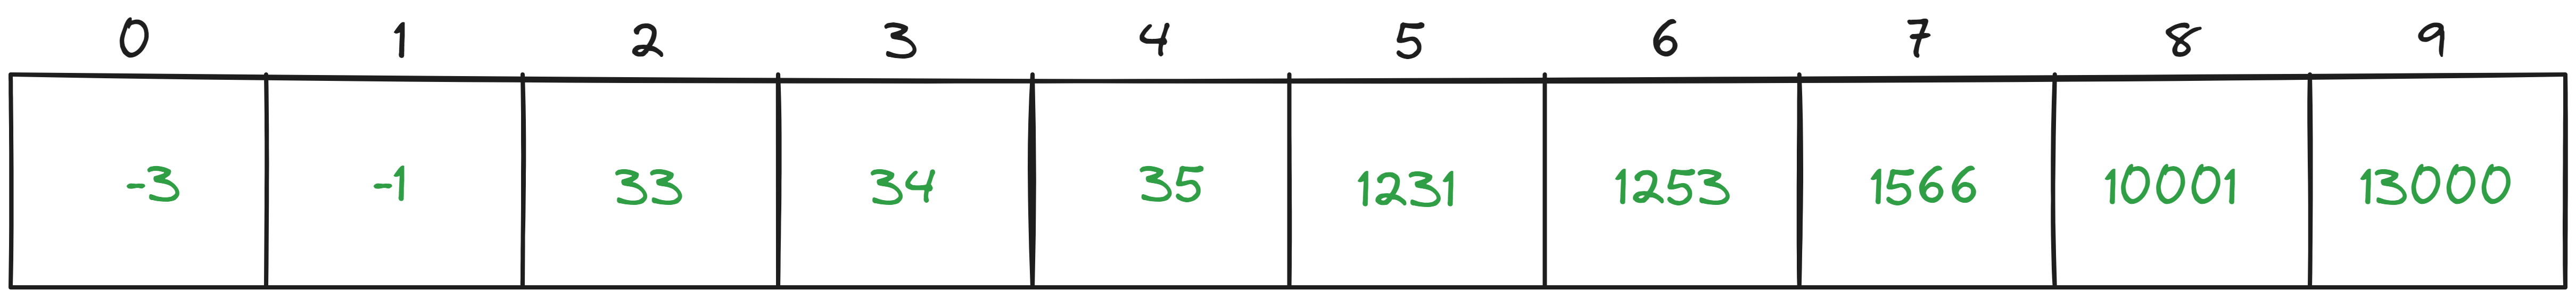
\includegraphics[width=\textwidth]{arreglo_inicial_busqueda.png}
\end{frame}

\begin{frame}[fragile]{Buscar un elemento: búsqueda lineal}
    En la mayoría de los casos, cuando necesitemos buscar un elemento dentro de un arreglo implementaremos una \alert{búsqueda lineal}
\begin{lstlisting}[basicstyle=\scriptsize]
// busqueda lineal
void buscarChar(const char arr[], int tam, char c) {
    int i = 0;
    bool encontrado = false;
    while(i<tam && !encontrado) {
        if (arr[i] == c)
            encontrado=true;
        i++;
    }

    if (encontrado)
        cout << "Encontre " << c << " en " << i-1 << endl;
    else
        cout << "No encontre el char " << c << endl;
}
\end{lstlisting}
\end{frame}

\begin{frame}{Buscar un elemento: búsqueda lineal}
    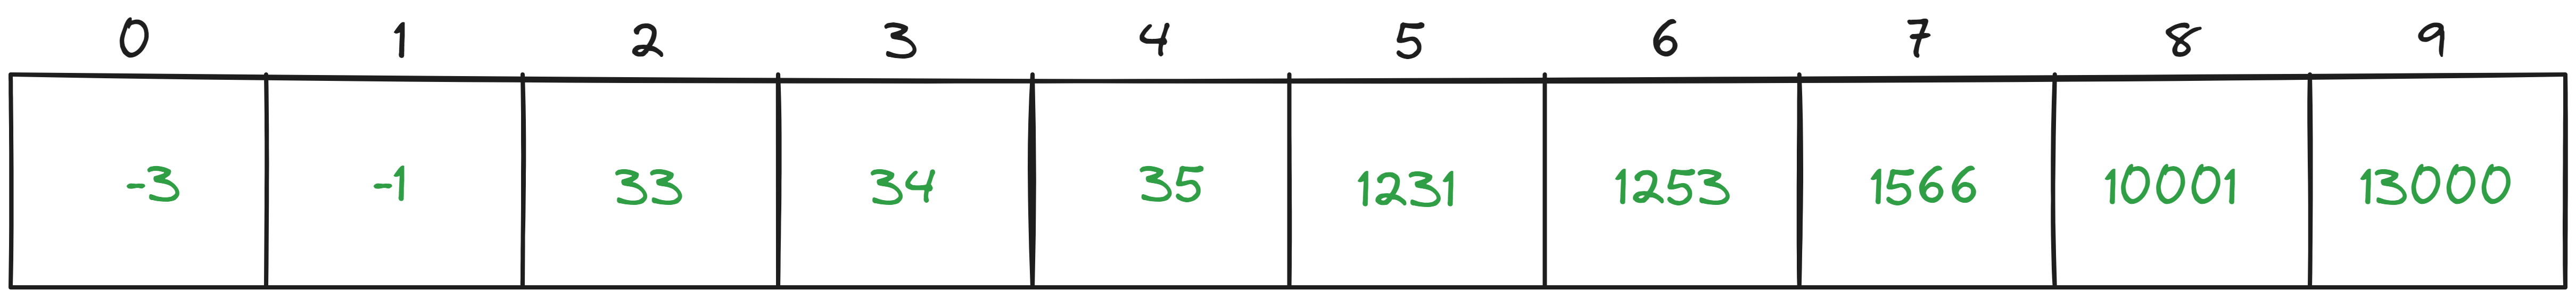
\includegraphics[width=\textwidth]{arreglo_inicial_busqueda.png}
\end{frame}

\begin{frame}{Buscar un elemento: búsqueda lineal}
    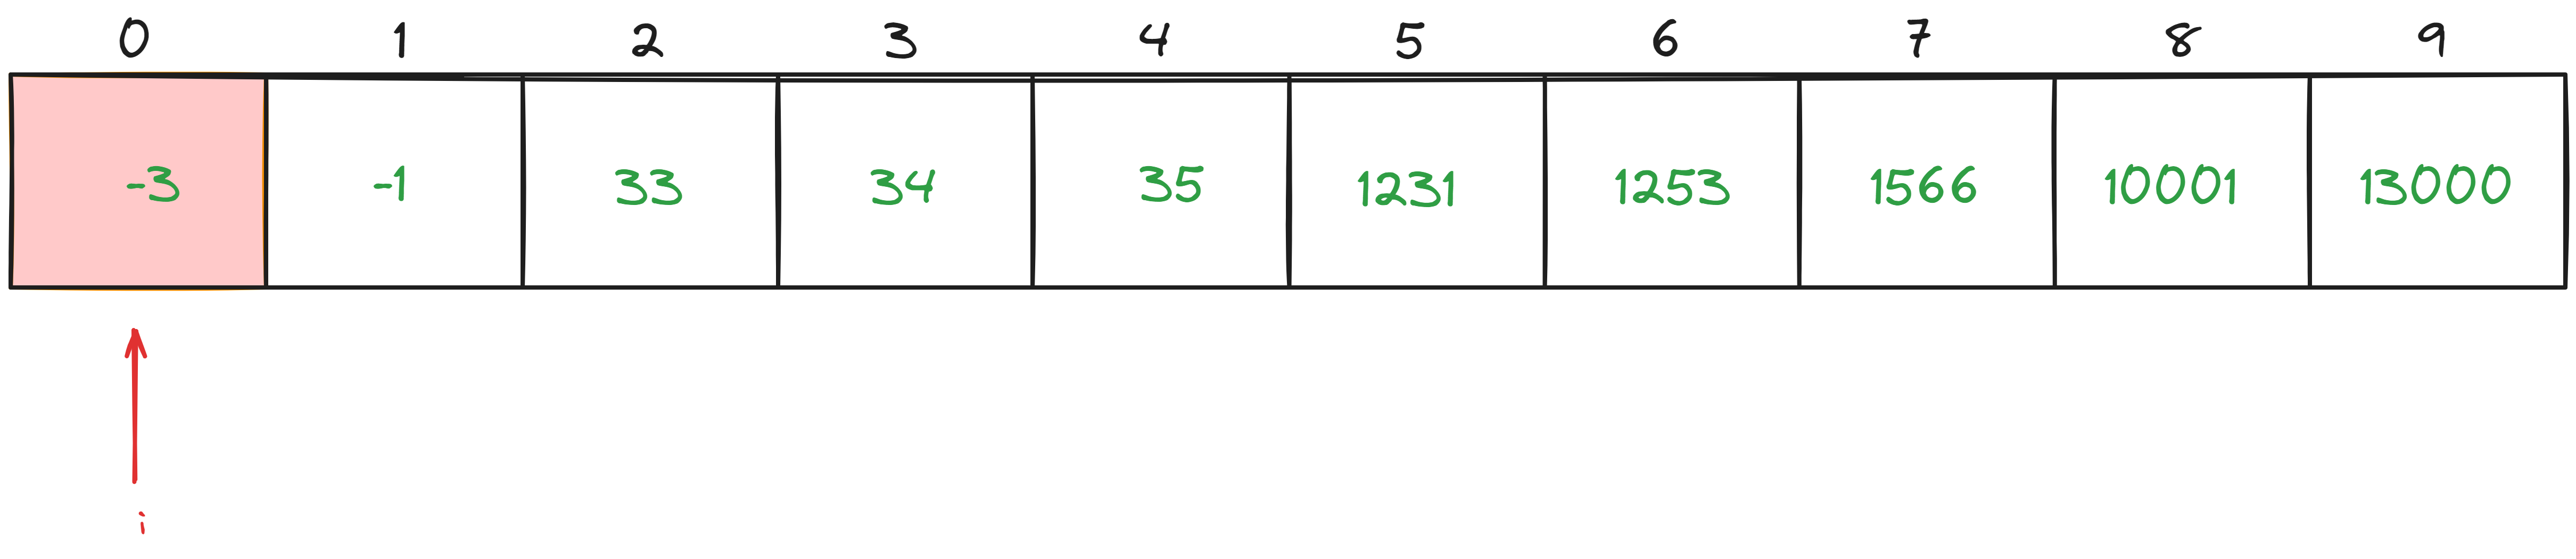
\includegraphics[width=\textwidth]{busqueda_lineal_1.png}
\end{frame}

\begin{frame}{Buscar un elemento: búsqueda lineal}
    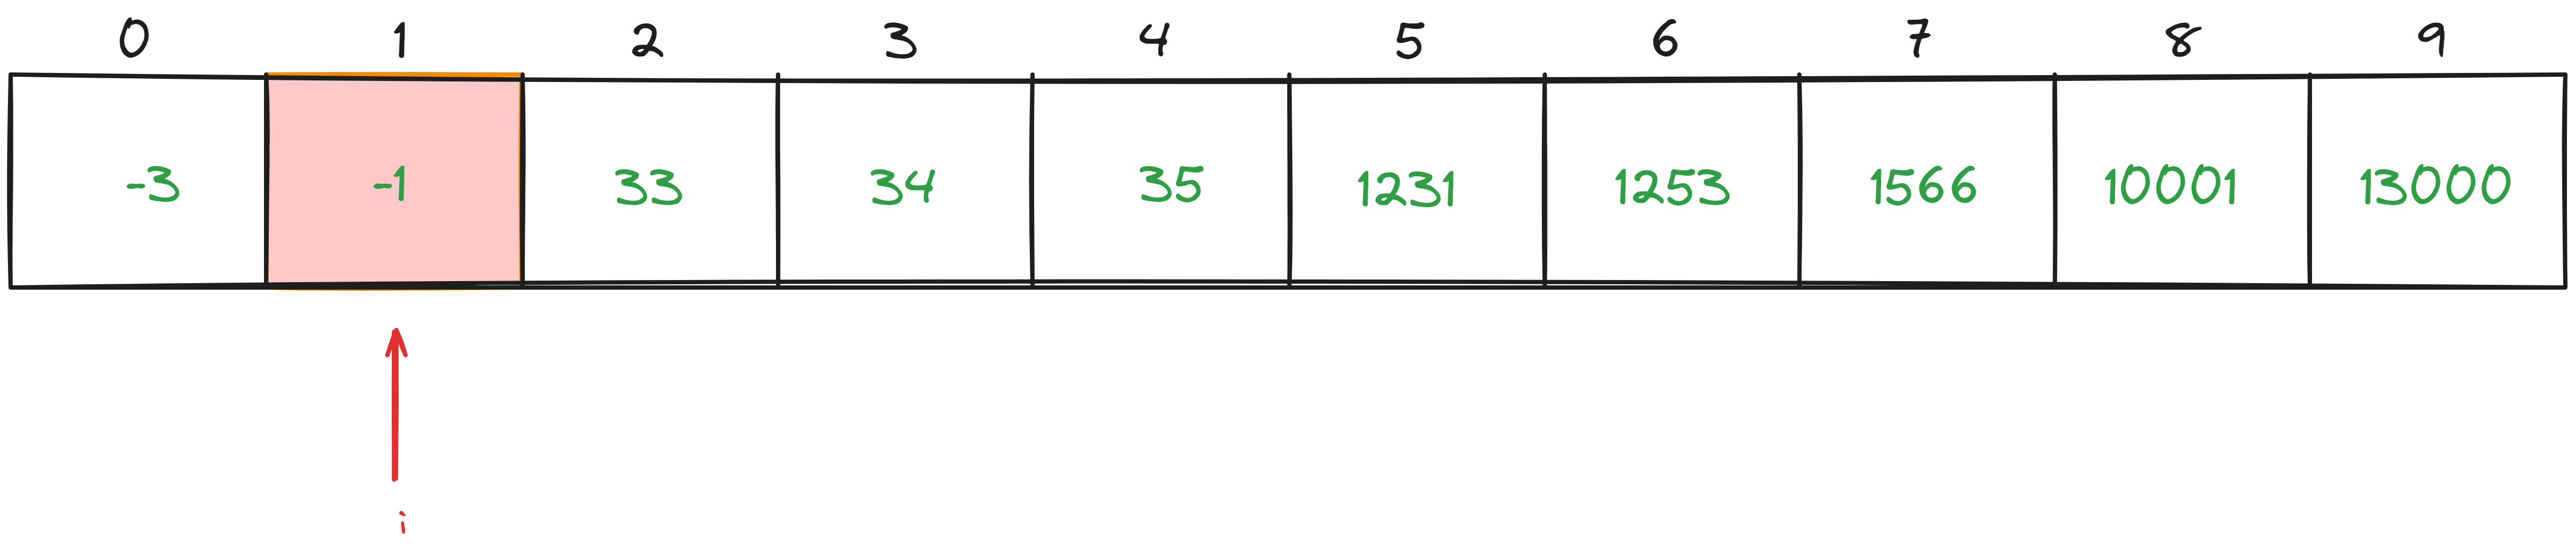
\includegraphics[width=\textwidth]{busqueda_lineal_2.png}
\end{frame}

\begin{frame}{Buscar un elemento: búsqueda lineal}
    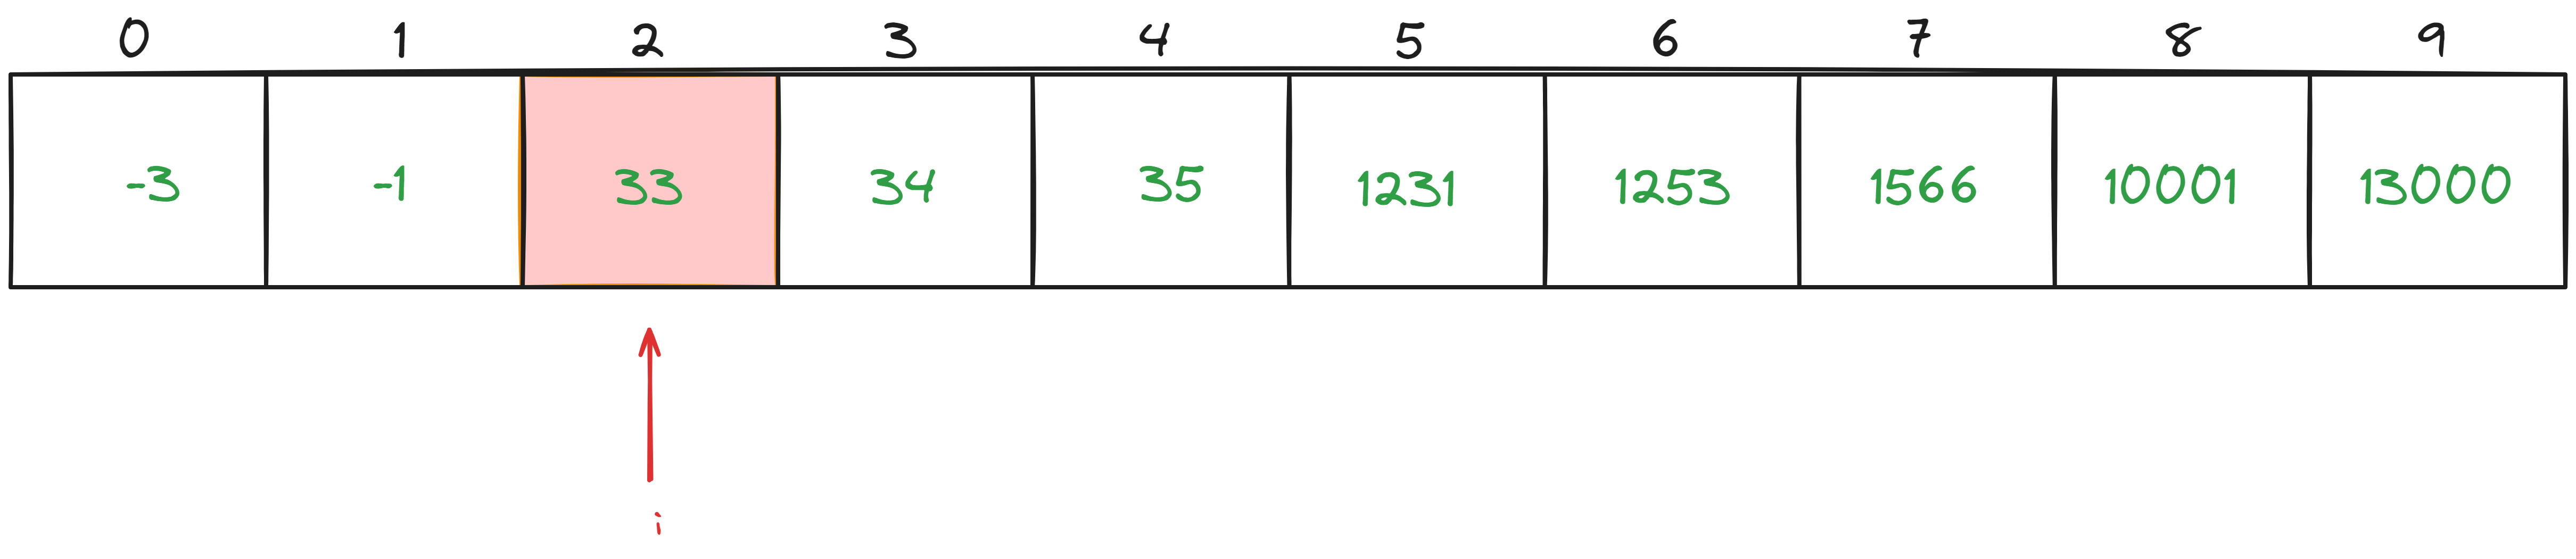
\includegraphics[width=\textwidth]{busqueda_lineal_3.png}
\end{frame}

\begin{frame}{Buscar un elemento: búsqueda lineal}
    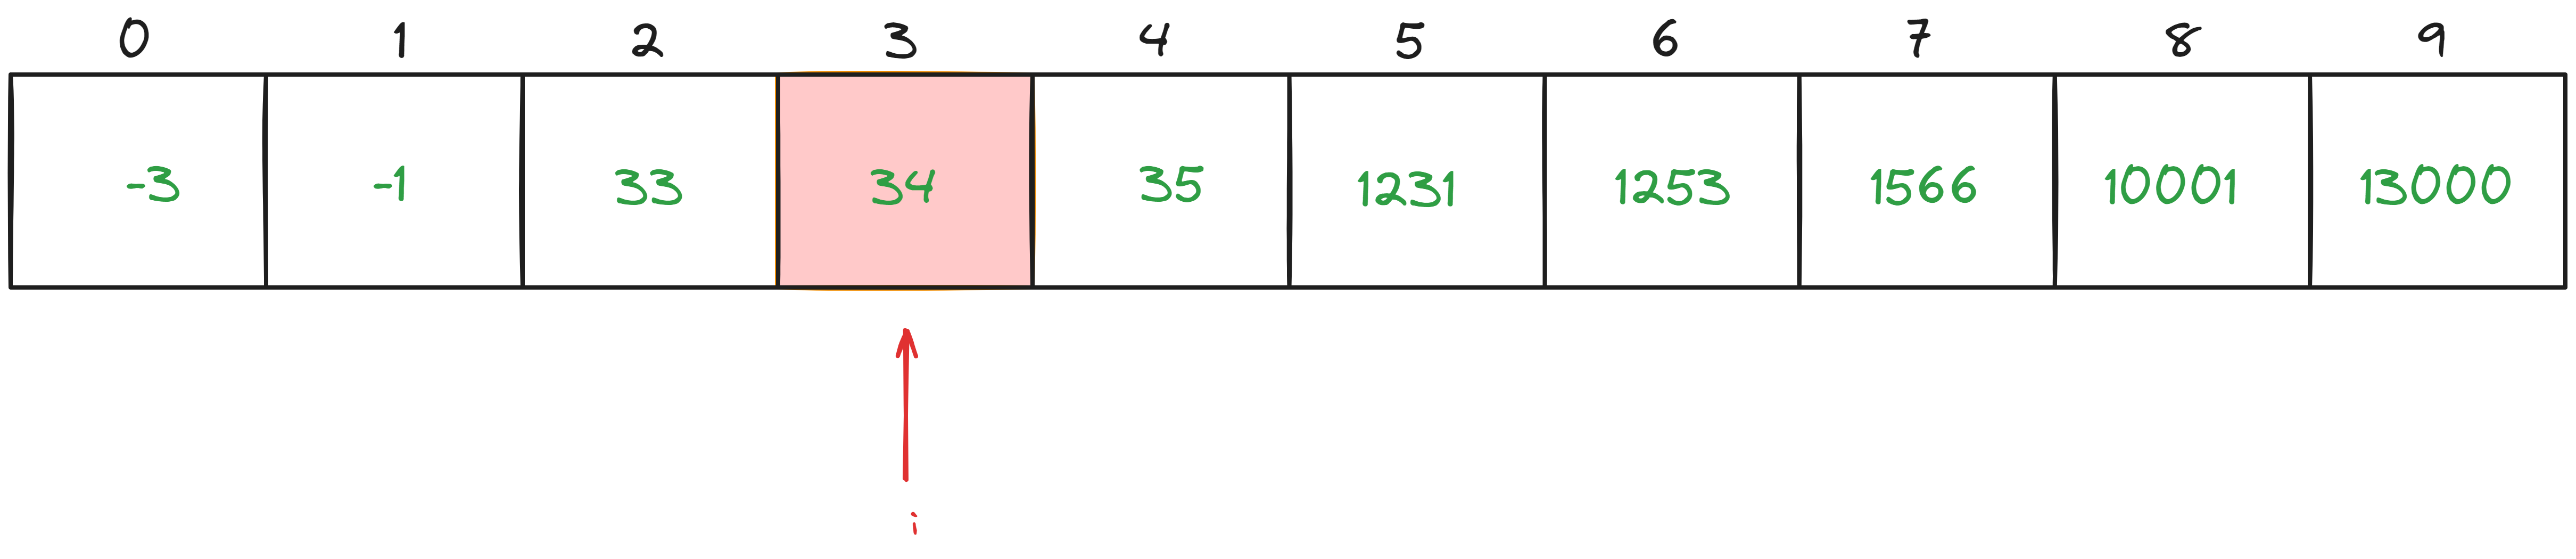
\includegraphics[width=\textwidth]{busqueda_lineal_4.png}
\end{frame}

\begin{frame}{Buscar un elemento: búsqueda lineal}
    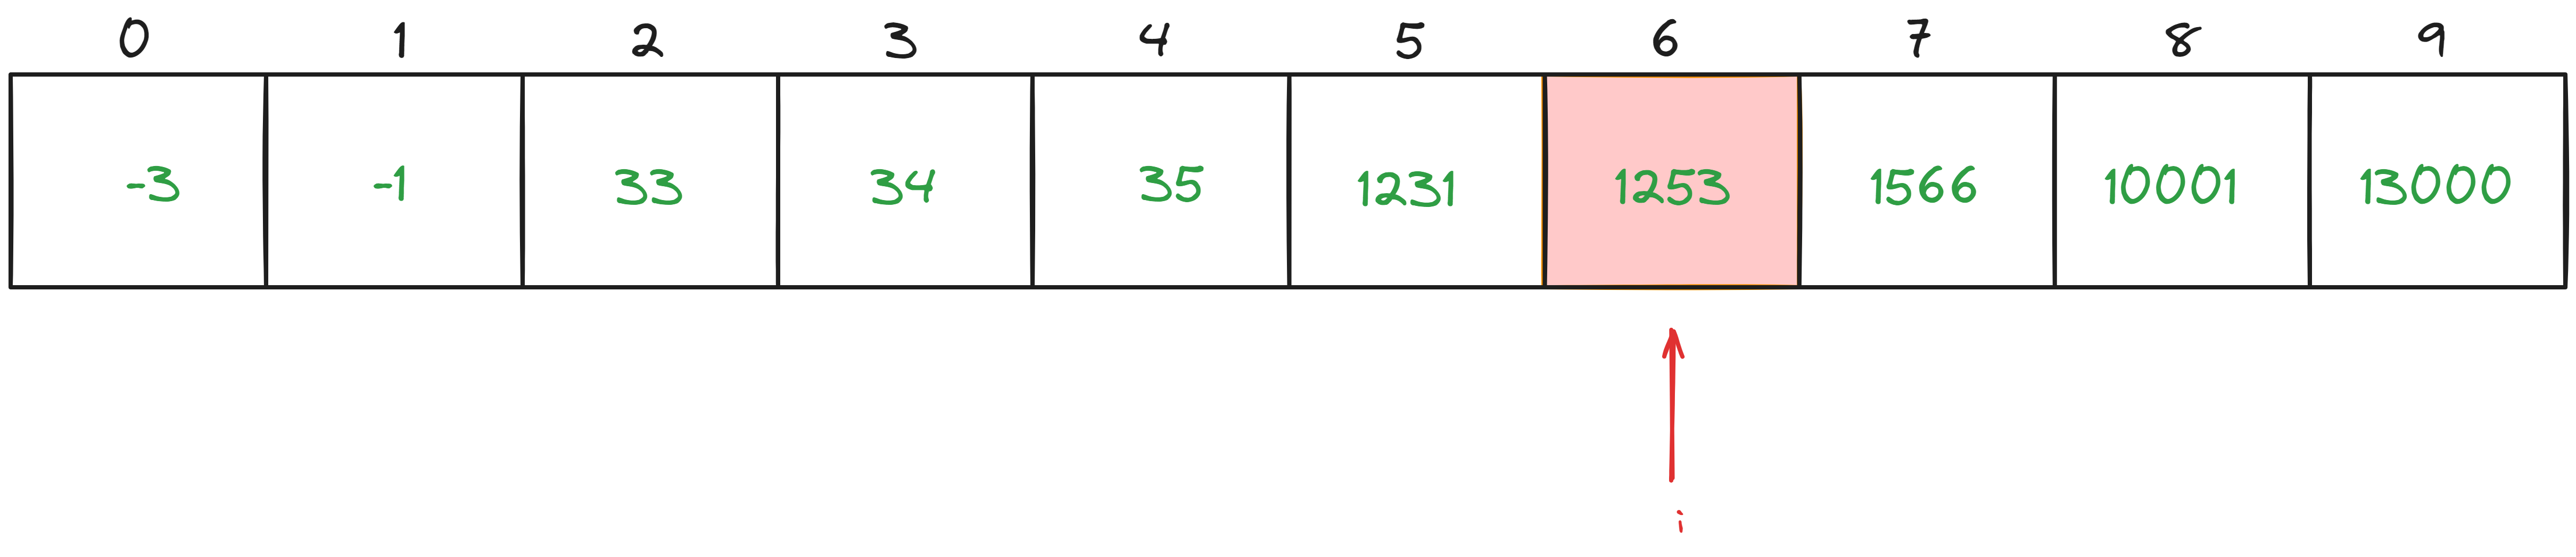
\includegraphics[width=\textwidth]{busqueda_lineal_final.png}
\end{frame}

\begin{frame}{Buscar un elemento: búsqueda lineal}
    La \alert{búsqueda lineal} es un algoritmo simple de implementar y que aplica para gran variedad de casos. Pero, qué ocurre si el arreglo sobre el que estamos realizando la búsqueda tiene 100 millones de elementos?
\end{frame}

\begin{frame}{Buscar un elemento: búsqueda lineal}
    La \alert{búsqueda lineal} es un algoritmo simple de implementar y que aplica para gran variedad de casos. Pero, qué ocurre si el arreglo sobre el que estamos realizando la búsqueda tiene 100 millones de elementos?
    
    \medskip

    \begin{center}
        
\includegraphics[width=0.7\textwidth]{skeleton_meme.jpg}
    \end{center}
\end{frame}

\begin{frame}[fragile]{Buscar un elemento: búsqueda binaria}
    Para los casos en donde el arreglo se encuentre \alert{ordenado}, podemos aplicar una búsqueda binaria
\begin{lstlisting}[basicstyle=\tiny]
// buscar de una manera mas eficiente, rapida.....
// -> busqueda binaria
// (solo se puede aplicar si el arreglo se encuentra ordenado)
// retorna la posicion en la que se encuentra el numero buscado
int buscarNumero(const int arr[], int tl, int num) {
	int izq = 0, der = tl-1;
	int medio;
	bool encontrado = false;
	while(izq<=der && !encontrado) {
		
		medio = (izq+der)/2;
		
		if (arr[medio] == num) {
			encontrado = true;
		}
		else if (arr[medio] > num) {
			der = medio - 1;
		}
		else {
			izq = medio + 1;
		}
	}
	
	return encontrado ? medio : -1;
}
\end{lstlisting}
\end{frame}

\begin{frame}[fragile]{Buscar un elemento: búsqueda binaria}
\begin{lstlisting}[basicstyle=\tiny]
int buscarNumero(const int arr[], int tl, int num) {
    int izq = 0, der = tl-1;
    int medio;
    bool encontrado = false;
    while(izq<=der && !encontrado) {
        
        medio = (izq+der)/2;
        
        if (arr[medio] == num) {
            encontrado = true;
        }
        else if (arr[medio] > num) {
            der = medio - 1;
        }
        else {
            izq = medio + 1;
        }
    }
    
    return encontrado ? medio : -1;
}
\end{lstlisting}
    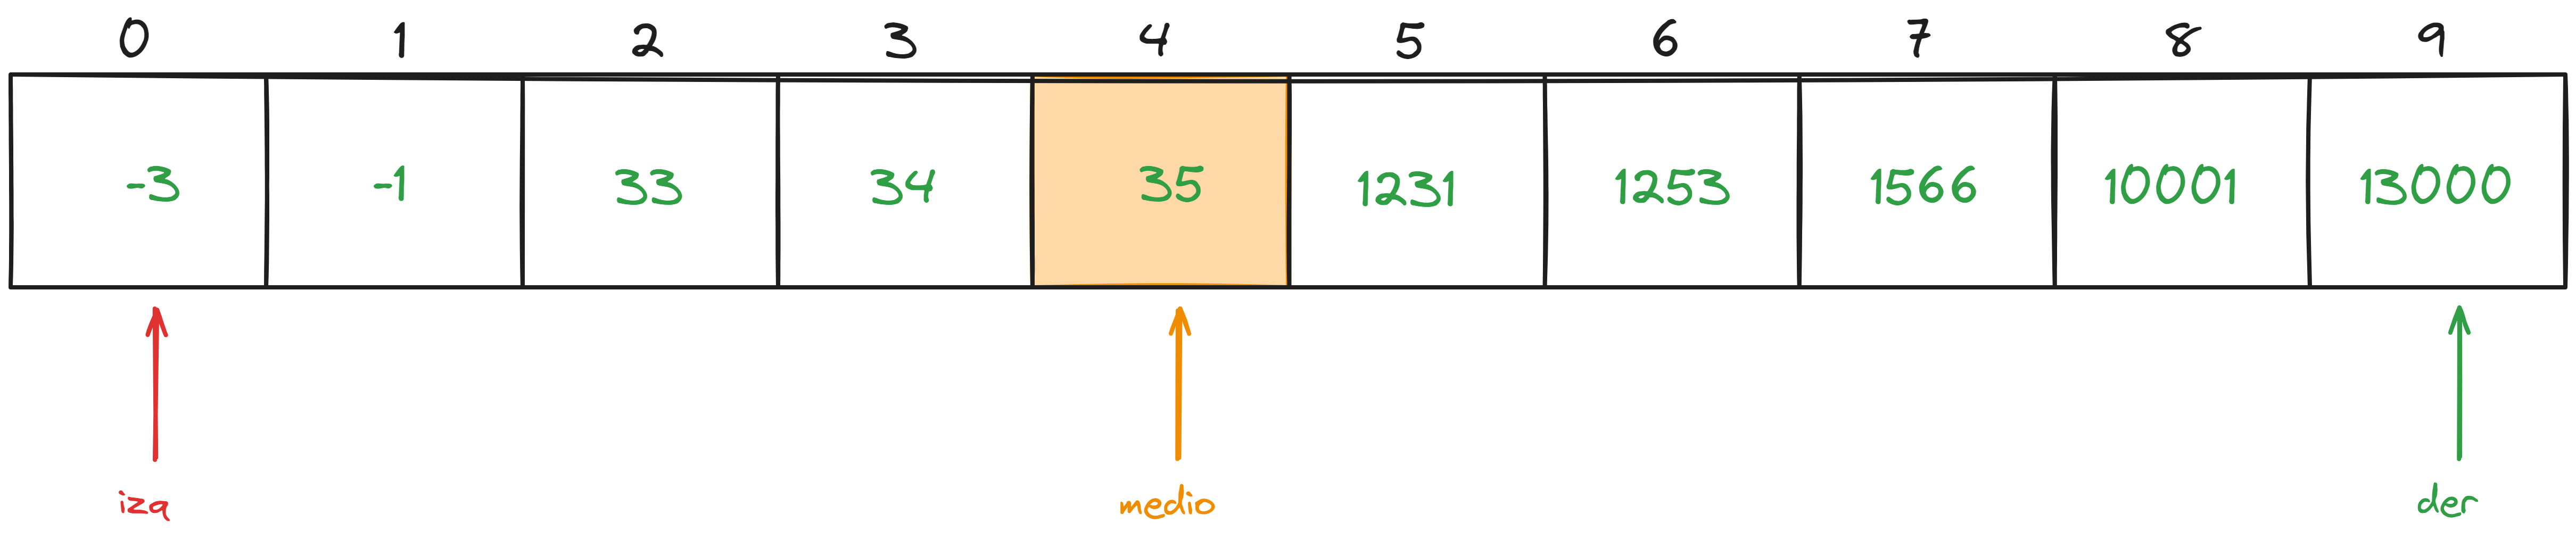
\includegraphics[width=\textwidth]{busqueda_binaria_1.png}
\end{frame}

\begin{frame}[fragile]{Buscar un elemento: búsqueda binaria}
\begin{lstlisting}[basicstyle=\tiny]
int buscarNumero(const int arr[], int tl, int num) {
    int izq = 0, der = tl-1;
    int medio;
    bool encontrado = false;
    while(izq<=der && !encontrado) {
        
        medio = (izq+der)/2;
        
        if (arr[medio] == num) {
            encontrado = true;
        }
        else if (arr[medio] > num) {
            der = medio - 1;
        }
        else {
            izq = medio + 1;
        }
    }
    
    return encontrado ? medio : -1;
}
\end{lstlisting}
    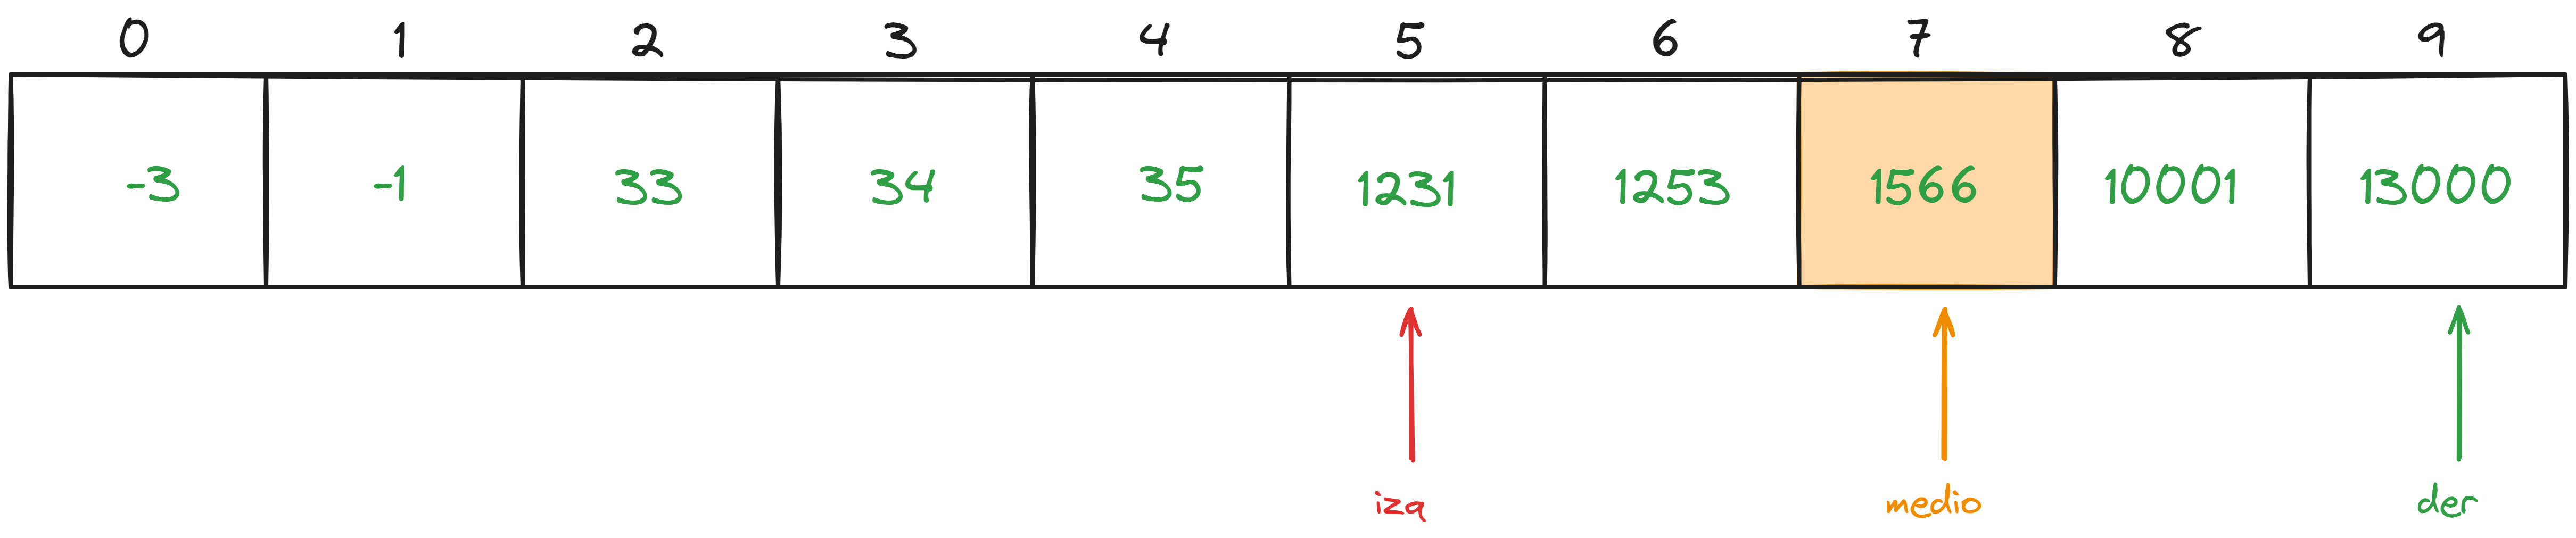
\includegraphics[width=\textwidth]{busqueda_binaria_2.png}
\end{frame}

\begin{frame}[fragile]{Buscar un elemento: búsqueda binaria}
\begin{lstlisting}[basicstyle=\tiny]
int buscarNumero(const int arr[], int tl, int num) {
    int izq = 0, der = tl-1;
    int medio;
    bool encontrado = false;
    while(izq<=der && !encontrado) {
        
        medio = (izq+der)/2;
        
        if (arr[medio] == num) {
            encontrado = true;
        }
        else if (arr[medio] > num) {
            der = medio - 1;
        }
        else {
            izq = medio + 1;
        }
    }
    
    return encontrado ? medio : -1;
}
\end{lstlisting}
    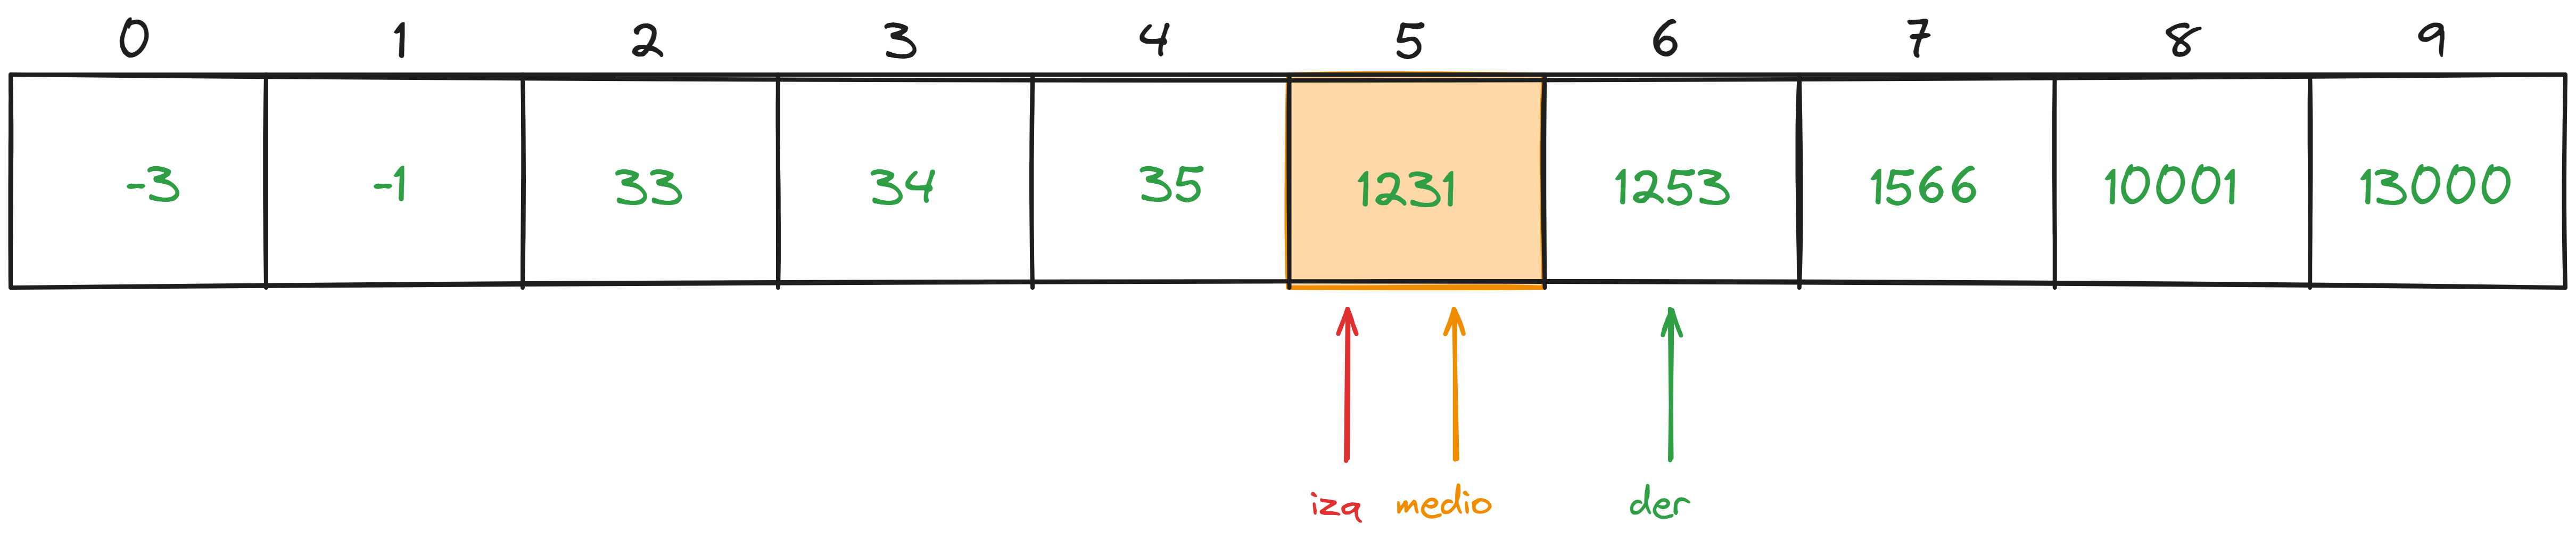
\includegraphics[width=\textwidth]{busqueda_binaria_3.png}
\end{frame}

\begin{frame}[fragile]{Buscar un elemento: búsqueda binaria}
\begin{lstlisting}[basicstyle=\tiny]
int buscarNumero(const int arr[], int tl, int num) {
    int izq = 0, der = tl-1;
    int medio;
    bool encontrado = false;
    while(izq<=der && !encontrado) {
        
        medio = (izq+der)/2;
        
        if (arr[medio] == num) {
            encontrado = true;
        }
        else if (arr[medio] > num) {
            der = medio - 1;
        }
        else {
            izq = medio + 1;
        }
    }
    
    return encontrado ? medio : -1;
}
\end{lstlisting}
    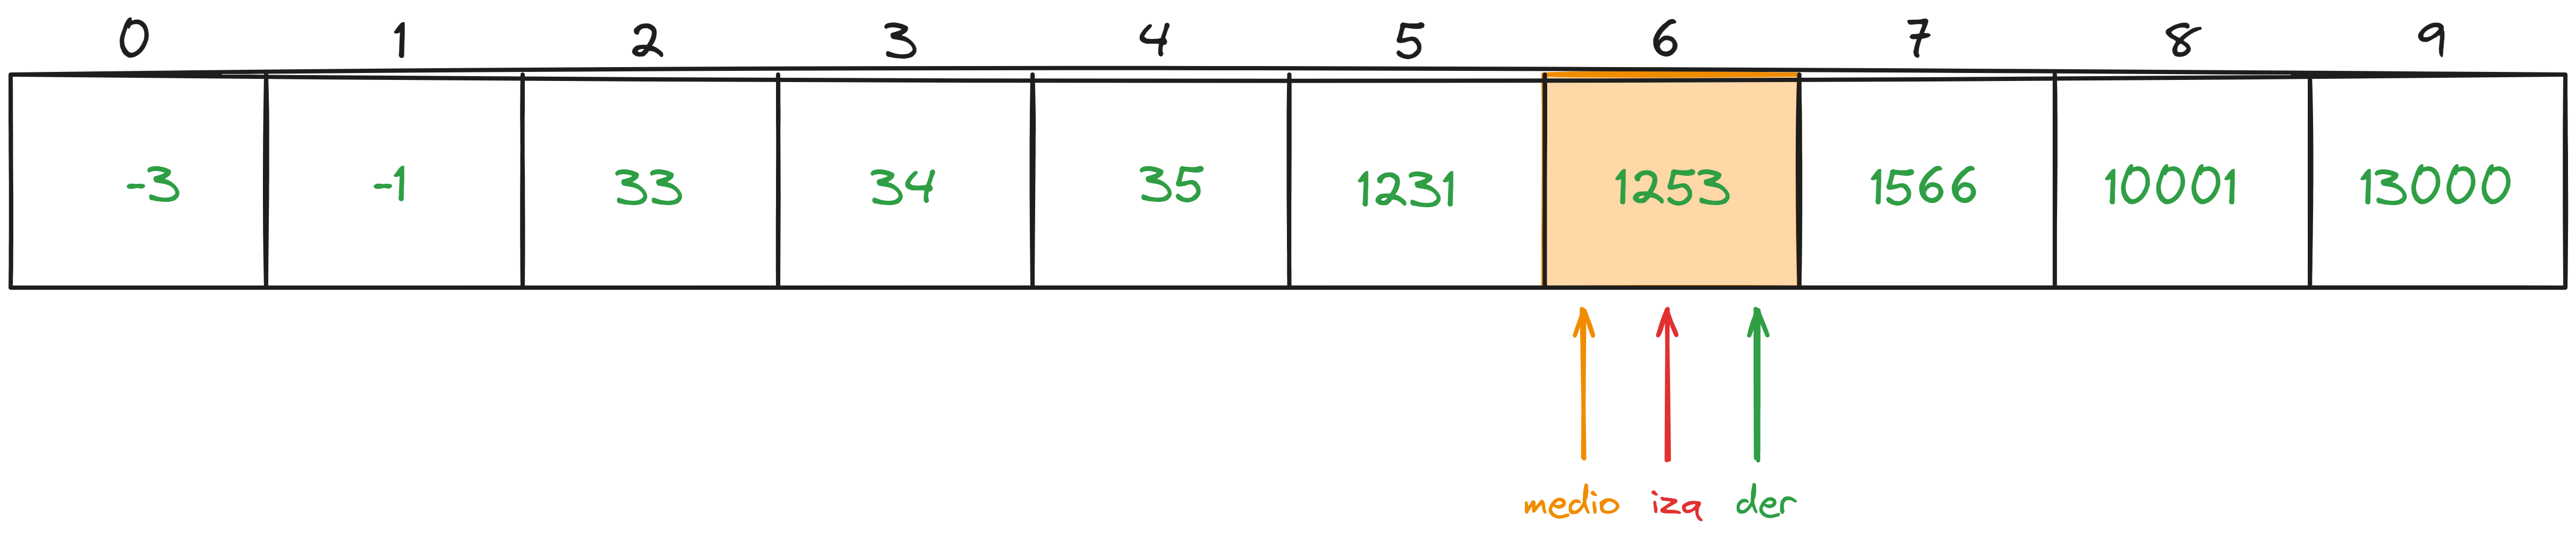
\includegraphics[width=\textwidth]{busqueda_binaria_final.png}
\end{frame}

\begin{frame}{Ordenamiento}
    Existen múltiples algoritmos de ordenamiento que pueden aplicarse sobre un arreglo, entre ellos se encuentran:
    \begin{itemize}
        \item BubbleSort (ordenamiento burbuja)
        \item SelectionSort (ordenamiento por selección)
        \item MergeSort
        \item Y más.... (que no los veremos)
    \end{itemize} 
    De todas formas, para la resolución de ejercicios basta con conocer bien uno. ¿Cuál? el que les resulte más sencillo de entender e implementar.

    \medskip

    \begin{center}
        \url{https://visualgo.net/en/sorting}
    \end{center}
\end{frame}

\begin{frame}[fragile]{Ordenamiento: BubbleSort}
\begin{lstlisting}[basicstyle=\scriptsize]
// ordenar de menor a mayor
void bubbleSort(char arr[], int tam) {
    for (int i = 0; i < tam; i++) {
        for (int j = 0; j < tam-1; j++) {
            if (arr[j] > arr[j + 1])
                swap(arr[j], arr[j + 1]);
            }
    }
}

// ordenar de mayor a menor
void bubbleSort2(char arr[], int tam) {
    for (int i = 0; i < tam; i++) {
        for (int j = 0; j < tam-1; j++) {
            if (arr[j] < arr[j + 1])
                swap(arr[j], arr[j + 1]);
            }
    }
}
\end{lstlisting}
\end{frame}

\begin{frame}[fragile]{Ordenamiento: SelectionSort}
    \begin{lstlisting}[basicstyle=\tiny]
// ordenar de menor a mayor
void selectionSort(int arr[], int tam) {
    for (int i = 0; i < tam; i++) {
        int indiceMenor=-1;
        for (int j = i; j < tam; j++) {
            if (indiceMenor == -1 || arr[j] < arr[indiceMenor])
                indiceMenor = j;
        }
        swap(arr[i], arr[indiceMenor]);
    }
}

// ordenar de mayor a menor
void selectionSort2(int arr[], int tam) {
    for (int i = 0; i < tam; i++) {
        int indiceMayor=-1;
        for (int j = i; j < tam; j++) {
            if (indiceMayor == -1 || arr[j] > arr[indiceMayor])
                indiceMayor = j;
        }
        swap(arr[i], arr[indiceMayor]);
    }
}
\end{lstlisting}
\end{frame}

\begin{frame}[fragile]{Ordenamiento: MergeSort}
\begin{lstlisting}[basicstyle=\tiny]
// divide el arreglo en dos subarreglos, los ordena y los une
void mergeSort(int arr[], int l, int r) {
    if (l < r) {
        // m es el punto donde el array se divide en dos
        int m = l + (r - l) / 2;

        mergeSort(arr, l, m);
        mergeSort(arr, m + 1, r);

        // Unir los sub-arreglos ordenados
        merge(arr, l, m, r);
    }
}
\end{lstlisting}
   \begin{center}
        \url{https://www.programiz.com/dsa/merge-sort}
   \end{center}
\end{frame}

\begin{frame}[fragile]{Ordenamiento: MergeSort}
\begin{lstlisting}[basicstyle=\tiny]
void merge(int arr[], int p, int q, int r) {
    // Crear arreglos L = A[p..q] and M = A[q+1..r]
    int n1 = q - p + 1, n2 = r - q;
    int L[10000], M[10000];
    for (int i = 0; i < n1; i++)
        L[i] = arr[p + i];
    for (int j = 0; j < n2; j++)
        M[j] = arr[q + 1 + j];

    int i=0, j=0, k=p;
    // Hasta que no alcancemos el final de L or M procesamos ambos juntos
    while (i < n1 && j < n2) {
        if (L[i] <= M[j]) {
            arr[k] = L[i];
            i++;
        } else {
            arr[k] = M[j];
            j++;
        }
        k++;
    }
    // insertamos los elementos restantes en A[p..r]
    while (i < n1) {
        arr[k] = L[i];
        i++; k++;
    }
    while (j < n2) {
        arr[k] = M[j];
        j++; k++;
    }
}
\end{lstlisting}
\end{frame}

\end{document}